\documentclass[12pt,letterpaper]{article}
\usepackage{inverba}
\newcommand{\userName}{Cullyn Newman} 
\newcommand{\class}{BI 216} 
\newcommand{\institution}{Portland State University} 
\newcommand{\thetitle}{\hypertarget{home}{Lab 3 Addendum: Water Quality}}
\rfoot{\hyperlink{home}{\thepage}}

\begin{document}
\section*{Part A: Smithsonian Ocean}
\begin{enumerate}[font=\bfseries, wide]
    {\color{under}\item What does the figure just below the  “A More Acidic Ocean” figure illustrate? Please summarize the data in the figure (remember to account for all of the variables!) \textbf{(2pts)}}

    The figure shows the rising levels of \ch{CO2}, from approximately 320 ppm to over 380 ppm, in the atmosphere from 1960 to 2010; rising \ch{CO2}, from approximately 325 ppm to over 360 ppm, in the ocean from 1990 to 2010; and decreasing pH, from approximately 8.13 to under 8.08, in the water off the coast of Hawaii from 1990 to 2010.\par 

    To summarize, this graph is showing how increasing \ch{CO2} in the atmosphere is increasing \ch{CO2} in the ocean, which increases ocean acidity due to creation of carbonic acid when water and \ch{CO2} mix. 

    {\color{under}\item What does “ocean acidification” mean? \textbf{(1 pt)}}

    Ocean acidification is a significant and harmful consequence in which the pH of the ocean decreases due to the of excess carbon dioxide in the atmosphere. 

    {\color{under}\item How does the level of acidity in the ocean impact:}
    \begin{enumerate}
        {\color{under}\item  A bivalve’s shell development? \textbf{(0.5pts)}}

        Water with that is more acidic can dissolves shells and make it harder, if not nearly impossible, for shells to grow in the first place due to the organisms inability to extract the carbonate ion they need to form bicarbonate. 

        {\color{under}\item  A coral’s structure? \textbf{(0.5pts)}}

        Acidification may limit coral growth by corroding pre-existing coral skeletons and preventing growth of new ones. Weaker reefs are more vulnerable to erosion from storm waves and other animals that drill or eat the coral. 
    \end{enumerate}
    \newpage
    {\color{under}\item Follow the links, and work to find the actual article on the research on black-finned clownish which was described in the In the Lab section}
    \begin{enumerate}
        {\color{under}\item What is the name of the journal in which it was published, and what was the (print) publication date and year \textbf{(0.25pts)}}

        Published by Biology Letters, Dec 32, 2011.

        {\color{under}\item The study was novel because it showed that fish have the ability to respond to predator sounds when played underwater:  TRUE or FALSE \textbf{(0.25pts)}}

        False. This was already known, the study was novel because it showed that ocean acidification affects the response. 
    \end{enumerate}
\end{enumerate}

\section*{Part B: Measuring Salinity in Estuaries}
\subsection*{Level 3: Measuring Salinity in Estuaries}
\begin{enumerate}[font=\bfseries, wide, resume]
    {\color{under}\item Question \#5 from the activity: Which statement represents a valid conclusion based on the graph?  Enter the correct letter and the statement \textbf{(0.5pts)}}

    C. A rainstorm on Oct 25 may have caused the decrease in salinity on Oct 27

    {\color{under}\item What may have caused Delta Smelt to be found outside of their normal range? \textbf{(0.5pts)} }

    There was a significant amount of rainfall during the times the salinity was higher than 2, and salinity also spiked when ever rainfall increased. 
\end{enumerate}

\subsection*{Level 4 - Research Question: Predicting the Return of the Atlantic Sturgeon}
\begin{enumerate}[font=\bfseries, wide, resume]
    {\color{under}\item To get started, use the online Fact Sheet to select an estuary where Atlantic Sturgeon are found. Record the estuary name and location here:  \textbf{(0.5pts)}  }

    The location we chose was Chesapeake Bay, MD and the Otter Point Creek Station.
    \newpage 

    {\color{under}\item Write your research question in the space below. \textbf{(1pt)} }

    How does dissolved oxygen and water temperature change over the month of April over and how does it compare to the following years and would these parameters be optimal for spawning of Atlantic Sturgeon.

    {\color{under}\item Complete the table \textbf{(1pt)}}\

    \begin{table}[h]
        \centering
        \caption{Water Quality for Otter Point Creek for Month of April from 2017-2019.}
        \begin{tabular}{m{0.2\linewidth}m{0.1\linewidth}m{0.2\linewidth}m{0.35\linewidth}}
            \toprule
            Parameter & Year & Range & Optimality for Spawning\\
            \midrule
            Temperature & 2017 & \SI{7.6} - \SI{25.9}{\celsius} & {\color{Fresh1}Majority} of Month\\
            Temperature & 2018 & \SI{7.7} - \SI{25.3}{\celsius}  & {\color{Fresh1}Majority} of Month\\
            Temperature & 2019 & \SI{10.0} - \SI{23.9}{\celsius}  & {\color{Sun1}Minority} of Month\\
            Dissolved \ch{O2} & 2017 & \SI{5.6} - \SI{15.3}{mg\per L} & {\color{Fresh2}Entirety} of Month \\
            Dissolved \ch{O2} & 2018 & \SI{5.1} - \SI{11.9}{mg\per L} & {\color{Fresh2}Entirety} of Month \\
            Dissolved \ch{O2} & 2019 & \SI{6.9} - \SI{17.8}{mg\per L} & {\color{Fresh2}Entirety} of Month \\
            \bottomrule
            \end{tabular}
    \end{table}
    
    {\color{under}\item Can you identify a time period when the water temperature is within the range for the sturgeon to return? \textbf{(0.5pts)}}

    Majority of April had ideal temperatures, with only a few days spiking or falling below the optimal range. 

    {\color{under}\item What is the range of the other water quality parameters during that time period? \textbf{(0.5pts)}}

    See Table 1. Generally between optimal range of 13-\SI{17}{\celsius} though. 

    {\color{under}\item Can you identify a time period when all the conditions look right for the sturgeon to return to spawn? \textbf{(0.5pts)}}

    Given the two parameters we looked at, water temperature and dissolved oxygen, then most of April were ideal times were spawning. Although, while not recorded, salinity was no where near the optimal range for any location in Chesapeake Bay, MD. 

    \newpage 

    {\color{under}\item Do the same conditions occur around the same time, year after year? \textbf{(0.5pts)}}

    Based on the data we collected, only 2019 seemed out of range. Yet, even then there were optimal spawning periods in the month. Despite this, other nearby months also appeared to follow a similar trend. So yes, generally the conditions occur roughly around the same time. 
\end{enumerate}

\subsection*{Level 5: Work as a team to develop your own investigation}
\begin{enumerate}[font=\bfseries, wide, resume]
    {\color{under}\item Read through Level 5 on your own, and then work with your team to develop your research question. State your research question here: \textbf{(1 pt)}}

    How does inland distance from the coast affect levels of salinity?

    {\color{under}\item State your hypothesis: \textbf{(1 pt)}}

    Salinity increases as the distance to the ocean decreases.

    {\color{under}\item \textit{Make a Plan:} Make a lis below of the specific data you will need to answer the question \textbf{(1 pt)} }

    \begin{table}[h]
        \centering
        \caption{Salinity of water from various locations in Chesapeake Bay, VA.}
        \begin{tabular}{cccc}
            \toprule
             Location & Distance from Ocean & Range of Dates & Salinity  \\
            \midrule
            Sweethall Pier & Closest & April 4-30, 2017 & 0.1 - 5.5 PSU \\
            Taskinas Creek & Between &April 4-30, 2017 & 2.2 - 16.0 PSU \\
            Claybank & Furthest &April 4-30, 2017 & 9.4 - 20.4 PSU \\
            \bottomrule
            \end{tabular}
    \end{table}
    
    {\color{under}\item Other than the data listed above, what other information (if any) will you need to answer your question? \textbf{(1 pt)}}

    Exact distance was not provided in information, but relativity to each other was all that was really required to answer this hypothesis. 

    There could still be other factors (known or unknown) that influence salinity, so more data is needed to fully support the hypothesis. 
    \newpage
    {\color{under}\item Insert figure here \textbf{(1 pt)}}
        \begin{figure}[h]
            \centering
            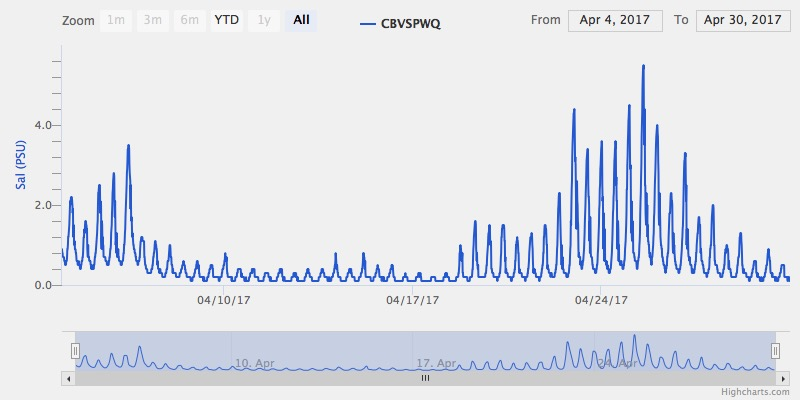
\includegraphics[width=0.5\linewidth]{images/Sweethall.jpeg}
            \caption{Salinity of Sweethall Pier from April 4-30, 2017}
        \end{figure}
        \begin{figure}[h]
            \centering
            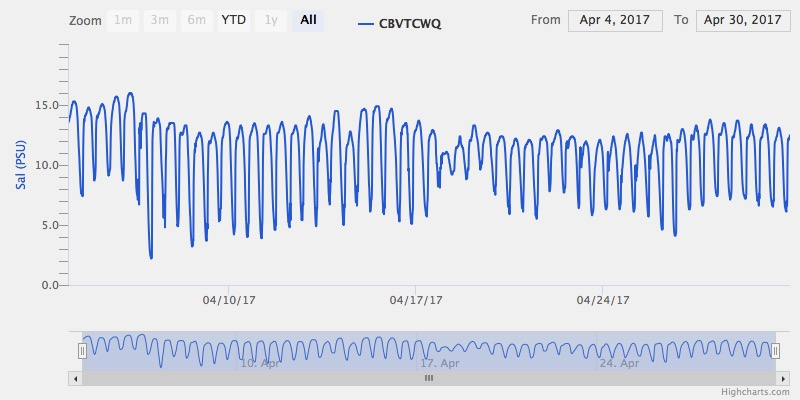
\includegraphics[width=0.5\linewidth]{images/Taskinas Creek.jpeg}
            \caption{Salinity of Taskinas Creek from April 4-30, 2017}
        \end{figure}
        \begin{figure}[h]
            \centering
            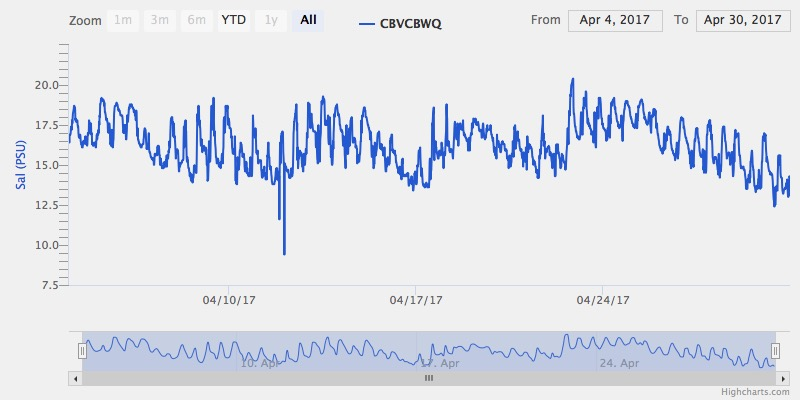
\includegraphics[width=0.5\linewidth]{images/Claybank.jpeg}
            \caption{Salinity of Claybank from April 4-30, 2017}
        \end{figure}
    {\color{under}\item \textit{Interpret the data:} What does your data show? Be specific and descriptive. Does the data support your hypothesis? \textbf{(1 pt)}}

    Our data shows than salinity actually decreases as distance to ocean decreases. This data rejects our hypothesis.

    \newpage
    {\color{under}\item \textit{Draw a Conclusion:} What is the answer to your question? Use evidence and data to support your conclusion. \textbf{(1 pt)}}
    
    Salinity increases as distance from the coast increases in Chesapeake Bay, VA given the data gathered from three stations monitoring water quality. 
    
    Sweethall Pier, the closest to the ocean, was barely above 1 PSU for over half the month, only spiking briefly. Meanwhile, Claybank almost consistently above 15 PSU, with Taskinas Creek showing periodic range between the two for the entirety of the month, but still less than Claybank. 

    This data suggested that salinity is very low in seawater, and water coming from inland is perhaps the source of increased salinity. 
    
    \subsubsection*{Additional Comprehension Questions}
    {\color{under}\item Give a specific example of why it would be biologically relevant to measure \textbf{temperature} in an aquatic environment. \textbf{(1 pt)}}

    You could be researching marine life as a whole in specific a aquatic environment and water temperature could greatly influence many functions of wide variety organisms. Observing changes in the ecosystem due to temperature changes would be very important to keep track of. 

    {\color{under}\item Give a specific example of why it would be biologically relevant to measure \textbf{dissolved oxygen} in an aquatic environment. \textbf{(1 pt)}}

    You could be researching shallow water fish, which require 4-15 mg/L dissolved \ch{O2} to thrive in the given water. 

    {\color{under}\item Give a specific example of why it would be biologically relevant to measure \textbf{carbon dioxide} in an aquatic environment. \textbf{(1 pt)}}

    You could be researching plants in an aquatic environment, which require carbon dioxide for photosynthesis. 
\end{enumerate}
\end{document}